\documentclass[11pt,onecolumn]{article}
\usepackage{booktabs, multirow} % for borders and merged ranges
\usepackage{amsmath,amssymb,graphicx,algorithmic,xspace,url}
\usepackage[titlenotnumbered,noend,noline]{algorithm2e}
\usepackage{enumerate}
\usepackage{mathrsfs}
\usepackage{color,soul}
\usepackage{array}
\usepackage{csquotes}
\usepackage{dirtytalk}



\setlength{\pdfpagewidth}{8.5in}
\setlength{\pdfpageheight}{11in}
\setlength{\evensidemargin}{-0.1in} \setlength{\oddsidemargin}{-0.1in}
\setlength{\textwidth}{6.5in} \setlength{\textheight}{9.0in}
\setlength{\topmargin}{-0.6in}

\sloppypar
\begin{document}

\begin{center}
\begin{Large}
ECE 493, Spring 2020, Assignment 1\\
Due: Friday June 19, 11:59pm
\end{Large}
\end{center}
\vspace{.2em}

\vspace{.2em}
\begin{center}
Submit to the UWaterloo Crowdmark site using the link you received via email.
Your answer can be handwritten converted to an electronic file by and scanner or camera; or the answers can be typed up in a word processor or LaTeX and submitted as a pdf.
\end{center}
\vspace{.2em}

\vspace{.2em}
\section{MDPs}

\begin{enumerate}
    \item Let $G_t = R_{t+1} + \gamma R_{t+2} + \ldots + \gamma^{T-1} R_{T}$. Suppose $\gamma = 0.5$ and the following sequence of rewards is received: $R_1$ = 1, $R_2$ = 2, $R_3$ = 5, $R_4$ = -2, $R_5$ = 2, and $T$ = 5. Solve for $G_0$, $G_1$, $G_2$, $G_3$, $G_4$, and $G_5$.
    \setlength{\parskip}{6pt}
    
    Definitions:
    \begin{itemize}
        \item $G_t = R_{t+1} + \gamma G_{t+1}$
        \item $G_T = 0$
    \end{itemize}
    \begin{equation}
        \begin{aligned}
            G_5 = 0
        \end{aligned}
    \end{equation}

    \begin{equation}
        \begin{aligned}
            G_4 & = R_{5} + \gamma G_{5} \\ 
            & = 2 + 0.5 * 0 \\
            & = 2
        \end{aligned}
    \end{equation}

    \begin{equation}
        \begin{aligned}
            G_3 & = R_{4} + \gamma G_{4} \\ 
            & = -2 + 0.5 * 2 \\
            & = -1
        \end{aligned}
    \end{equation}

    \begin{equation}
        \begin{aligned}
            G_2 & = R_{3} + \gamma G_{3} \\ 
            & = 5 + 0.5 * -1 \\
            & = 4.5
        \end{aligned}
    \end{equation}

    \begin{equation}
        \begin{aligned}
            G_1 & = R_{2} + \gamma G_{2} \\ 
            & = 2 + 0.5 * 4.5 \\
            & = 4.25
        \end{aligned}
    \end{equation}

    \begin{equation}
        \begin{aligned}
            G_0 & = R_{1} + \gamma G_{1} \\ 
            & = 1 + 0.5 * 4.25 \\
            & = 3.125
        \end{aligned}
    \end{equation}
    \item Let $G_t = \sum_{k=0}^\infty \gamma^k R_{t+k+1}$. Suppose $\gamma = 0.9$ and the reward sequence is $R_1 =2$, followed by an infinite sequence of 6s. What are $G_0$ and $G_1$?
    \setlength{\parskip}{6pt}
    
    Definitions:
    \begin{itemize}
        \item $\sum_{k=0}^{\infty} ar^k = \frac{a}{1-r}$ for $\vert r \vert < 1$
    \end{itemize}
    \begin{equation}
        \begin{aligned}
        G_1 & = \sum_{k=0}^\infty 0.9^k6\\
        & = \frac{6}{1-0.9}\\
        & = 60\\ 
        \end{aligned}
    \end{equation}

    \begin{equation}
        \begin{aligned}
        G_0 & = R_{1} + \gamma G_{1} \\ 
        & = 2 + 0.9*60\\
        & = 56\\ 
        \end{aligned}
    \end{equation}
    \item Suppose you treated pole-balancing as an episodic task but also used discounting, with all rewards zero except for -1 upon failure. What then would the return be at each time? How does this return differ from that in the discounted, continuing formulation of this task? (For explanation of pole-balancing see Example 3.4 on Sutton's RL Book)
    \setlength{\parskip}{6pt}

    The return at each instance will be $-\gamma ^{T-t-1}$. In contrast the continuous case has a reward at each time instance of $-\gamma^{K}$ where $K$ represents the number of time steps until failure from the current state. After receiving a failure, $K$ refers to the next failure for the continuous case. Comparing these two cases, it can be seen that the continuous case can be represented as a infinite sequence of this episodic task, where $T=K$ in each subsequence.
    
    \item Figure \ref{fig:book3.14} (left) shows a rectangular grid world representation of a simple finite MDP. The cells of the grid correspond to the states of the environment. At each cell, four actions are possible: north, south, east, and west, which deterministically cause the agent to move one cell in the respective direction on the grid. Actions that would take the agent off the grid leave its location unchanged, but also result in a reward of -1. Other actions result in a reward of 0, except those that move the agent out of the special states A and B. From state A, all four actions yield a reward of +10 and take the agent to A'. From state B, all actions yield a reward of +5 and take the agent to B'. 
    
    Assuming discount factor $\gamma=0.9$ and equal probabilities to all four actions, value functions seen in Figure \ref{fig:book3.14} (right) obtained. Show numerically that the Bellman expectation equation holds for the cell at the middle of top row, valued at +4.4, with respect to its four neighboring states, valued at +8.8, +2.3, +5.3 and off-grid (These numbers are accurate only to one decimal place.) (\textbf{Hint:} Try to understand what happens when agent takes action to north, off-grid)
    
\end{enumerate}

\begin{figure}[htbp]
    \centering
    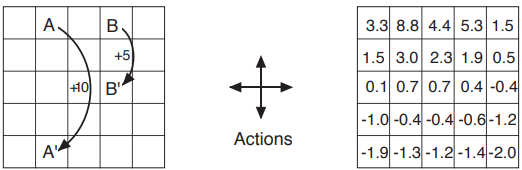
\includegraphics[width=0.6\linewidth]{figures/mdp_grid.png}
    
    \caption{Gridworld example: exceptional reward dynamics (left) and state-value function for the equiprobable random policy (right)}
    \label{fig:book3.14}
\end{figure}
\setlength{\parskip}{6pt}

Definitions:
\begin{itemize}
    \item $\upsilon_{\pi}(s) = \sum_{a} \pi(a \vert s) \sum_{s \prime, r}(s\prime, r \vert s, a)[r + \gamma\upsilon_{\pi}(s\prime)]$
\end{itemize}
Let's break the bellman expectation equation into it's components.
\begin{equation}
    \begin{aligned}
        \upsilon_{\pi}(s) & = \sum_{a} \pi(a \vert s) \sum_{s \prime, r}(s\prime, r \vert s, a)[r + \gamma\upsilon_{\pi}(s\prime)] \\
        & = \frac{0+0.9*8.8}{4}+\frac{0+0.9*5.3}{4} + \frac{0+0.9*2.3}{4} + \frac{-1+0.9*4.4}{4} \\ 
        & = 4.43 \\ 
        & = 4.4
    \end{aligned}
\end{equation}
\hl{$\therefore$ the Bellman expectation equation holds for the cell at the middle of the top row.}
\end{document}